% Options for packages loaded elsewhere
\PassOptionsToPackage{unicode}{hyperref}
\PassOptionsToPackage{hyphens}{url}
%
\documentclass[
]{book}
\usepackage{amsmath,amssymb}
\usepackage{iftex}
\ifPDFTeX
  \usepackage[T1]{fontenc}
  \usepackage[utf8]{inputenc}
  \usepackage{textcomp} % provide euro and other symbols
\else % if luatex or xetex
  \usepackage{unicode-math} % this also loads fontspec
  \defaultfontfeatures{Scale=MatchLowercase}
  \defaultfontfeatures[\rmfamily]{Ligatures=TeX,Scale=1}
\fi
\usepackage{lmodern}
\ifPDFTeX\else
  % xetex/luatex font selection
\fi
% Use upquote if available, for straight quotes in verbatim environments
\IfFileExists{upquote.sty}{\usepackage{upquote}}{}
\IfFileExists{microtype.sty}{% use microtype if available
  \usepackage[]{microtype}
  \UseMicrotypeSet[protrusion]{basicmath} % disable protrusion for tt fonts
}{}
\makeatletter
\@ifundefined{KOMAClassName}{% if non-KOMA class
  \IfFileExists{parskip.sty}{%
    \usepackage{parskip}
  }{% else
    \setlength{\parindent}{0pt}
    \setlength{\parskip}{6pt plus 2pt minus 1pt}}
}{% if KOMA class
  \KOMAoptions{parskip=half}}
\makeatother
\usepackage{xcolor}
\usepackage{longtable,booktabs,array}
\usepackage{calc} % for calculating minipage widths
% Correct order of tables after \paragraph or \subparagraph
\usepackage{etoolbox}
\makeatletter
\patchcmd\longtable{\par}{\if@noskipsec\mbox{}\fi\par}{}{}
\makeatother
% Allow footnotes in longtable head/foot
\IfFileExists{footnotehyper.sty}{\usepackage{footnotehyper}}{\usepackage{footnote}}
\makesavenoteenv{longtable}
\usepackage{graphicx}
\makeatletter
\def\maxwidth{\ifdim\Gin@nat@width>\linewidth\linewidth\else\Gin@nat@width\fi}
\def\maxheight{\ifdim\Gin@nat@height>\textheight\textheight\else\Gin@nat@height\fi}
\makeatother
% Scale images if necessary, so that they will not overflow the page
% margins by default, and it is still possible to overwrite the defaults
% using explicit options in \includegraphics[width, height, ...]{}
\setkeys{Gin}{width=\maxwidth,height=\maxheight,keepaspectratio}
% Set default figure placement to htbp
\makeatletter
\def\fps@figure{htbp}
\makeatother
\setlength{\emergencystretch}{3em} % prevent overfull lines
\providecommand{\tightlist}{%
  \setlength{\itemsep}{0pt}\setlength{\parskip}{0pt}}
\setcounter{secnumdepth}{5}
\usepackage{booktabs}
\usepackage{fancyhdr}
\pagestyle{fancy}


\usepackage{xstring}
\usepackage{catchfile}
\CatchFileDef{\HEAD}{.git/refs/heads/master}{}
\newcommand{\gitrevision}{%
  \StrLeft{\HEAD}{7}%
}


% center of header
\fancyhead[CO,CE]{}
% center of footer
\fancyfoot[CO,CE]{\gitrevision}
% page number on the left of even pages and right of odd pages
\fancyfoot[LE,RO]{\thepage}


\ifLuaTeX
  \usepackage{selnolig}  % disable illegal ligatures
\fi
\usepackage[]{natbib}
\bibliographystyle{plainnat}
\usepackage{bookmark}
\IfFileExists{xurl.sty}{\usepackage{xurl}}{} % add URL line breaks if available
\urlstyle{same}
\hypersetup{
  pdftitle={FlowMax-Q Manual},
  pdfauthor={Srirama Bhamidipati},
  hidelinks,
  pdfcreator={LaTeX via pandoc}}

\title{FlowMax-Q Manual}
\author{Srirama Bhamidipati}
\date{Last Updated 2024-03-08 16:00:14 Asia/Calcutta}

\begin{document}
\maketitle

{
\setcounter{tocdepth}{1}
\tableofcontents
}
\chapter*{Preface}\label{preface}
\addcontentsline{toc}{chapter}{Preface}

This manual\footnote{Version \textbf{15b24d1}} is divided into two parts. Part I deals with handling FlowMax network (nodes and edges) in a QGIS environemnt and Part II deals with using the FlowMax-Q, a QGIS plugin to work with outputs from FlowMax.

\part{Editing in QGIS}\label{part-editing-in-qgis}

\chapter{Introduction}\label{introduction}

\begin{itemize}
\tightlist
\item
  Economy based scenarios are to be modified in the trade-databases.
\item
  Resilience based scenarios (GIS) fall into 2 categories:

  \begin{itemize}
  \tightlist
  \item
    node-based

    \begin{itemize}
    \tightlist
    \item
      editing geometries;
    \item
      editing attributes
    \end{itemize}
  \item
    edge-based

    \begin{itemize}
    \tightlist
    \item
      editing geometries;
    \item
      editing attributes
    \end{itemize}
  \end{itemize}
\item
  Technology based scenarios will affect the demand (freight composition)
\item
  Policy based scenarios will affect the route and mode choices (freight composition)
\end{itemize}

\chapter{Scenarios}\label{scenarios}

The image below shows the underlying structure of constructing scenarios

\begin{figure}
\centering
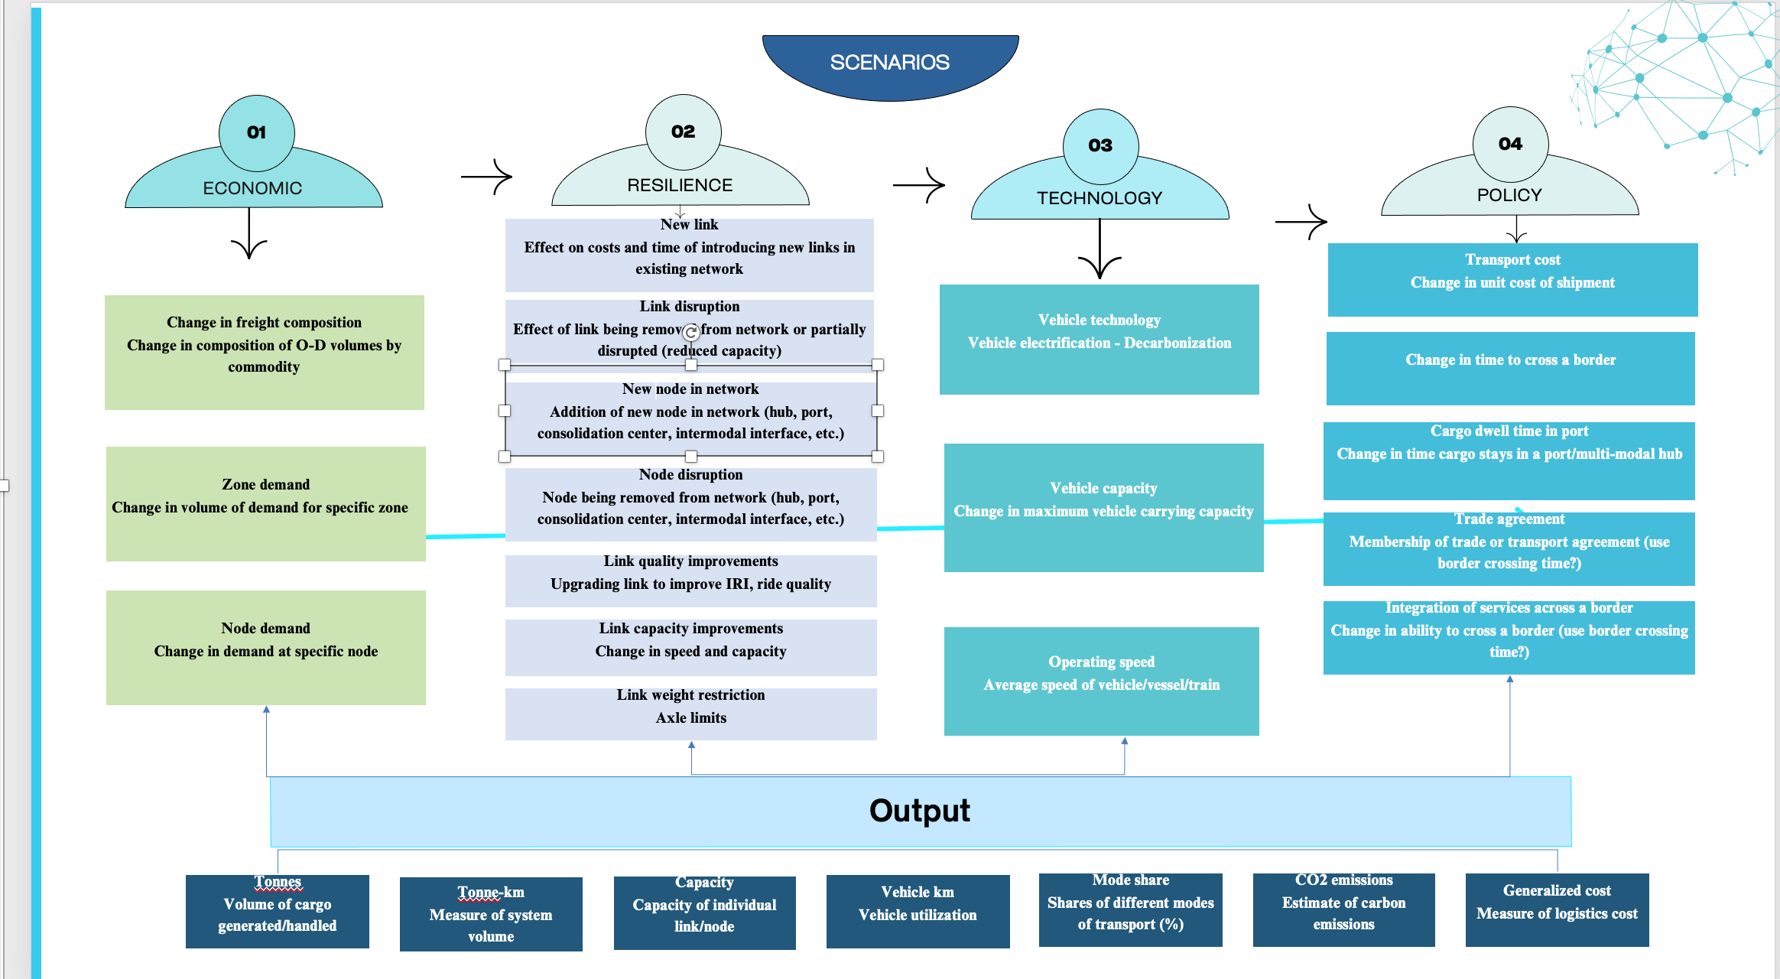
\includegraphics{images/Picture1.png}
\caption{Scenarios}
\end{figure}

\chapter{Adding Links}\label{adding-links}

\section{Connect to an non-existing node}\label{connect-to-an-non-existing-node}

Is there an existing node at the source or destination of this (to be added) new link?

\begin{itemize}
\tightlist
\item
  No? First create a node(s) and then create a line between source and destination nodes.
\item
  Yes ? Create a line between source and destination nodes.
\end{itemize}

\section{Connect to an existing node}\label{connect-to-an-existing-node}

Is the new link connecting to an existing node location?

\begin{itemize}
\tightlist
\item
  Create a line between source and destination nodes.
\end{itemize}

\section{Hands-on}\label{hands-on}

\subsection{Adding a New Link from an existing node}\label{adding-a-new-link-from-an-existing-node}

\begin{enumerate}
\def\labelenumi{\arabic{enumi}.}
\tightlist
\item
  Check the highest node number (NodeID\textsubscript{H}) from the node file. To do this, open the attribute table of the shapefile \textbf{Right Click on the node layer\textgreater{} Open Attribute Table} . Scroll if required to see the NodeID field, \textbf{Click on the field heading} to sort the column in ascending or descending order. When in descending order, make note of the top most row to identify the current highest node number.
\item
  Set the node file in edit mode, and add a node (point geometry) to the node file and assign it a node number = NodeID\textsubscript{H}+1
  - Fill in all other node attribute columns as necessary (\hyperref[modifying-node-attributes]{see how})
\item
  Save edits and stop the edit mode on node file.
\item
  Check the highest edge number (EdgeID\textsubscript{H}) from the link file.
\item
  Set the link file in edit mode and add a link (line-geometry) from existing node to the new node created in step 2, assign this link an edge number = EdgeID\textsubscript{H} + 1
  - Fill in all other link attribute columns as necessary (\hyperref[modifying-edge-attributes]{see how})
\item
  Save edits and stop the edit mode on link file
\end{enumerate}

\subsection{Adding a New Link from an existing link}\label{adding-a-new-link-from-an-existing-link}

\begin{enumerate}
\def\labelenumi{\arabic{enumi}.}
\tightlist
\item
  Check the highest node id (NodeID\textsubscript{H}) from the node file.
\item
  Set the node file in edit mode, and add a node (point geometry) to the node file at the required location on an existing link and assign it a node number = NodeID\textsubscript{H}+1
  - Fill in all other node attribute columns as necessary (\hyperref[modifying-node-attributes]{see how})
\item
  Save edits and stop the edit mode on node file.
\item
  Split the existing link at this new node from step 2.
  - When you split the link into two, the first part can retain existing edgeID but the second part needs a new edgeID.
\item
  Check the highest edgeID number (EdgeID\textsubscript{H}) from the link file.
\item
  Set the link file in edit mode and assign this second part link an edgeID = EdgeID\textsubscript{H} + 1
  - Fill in all other link attribute columns as necessary (\hyperref[modifying-edge-attributes]{see how})
\item
  Save edits and stop the edit mode on link file
\end{enumerate}

\chapter{Removing Links}\label{removing-links}

Removing links is easier than adding links. It is recommended to disable links than to delete them.

\section{Removing a Link (disabling links)}\label{removing-a-link-disabling-links}

It is advised not to remove a link (line-geometry) in GIS. It is recommended that you use the \texttt{active} attribute in the link shapefile:

\begin{itemize}
\item
  edit this attribute to a value 0 (integer) instead of a value 1(integer) for the link in consideration.
\item
  Assigning a 0 will add the current link to a set of inactive links i.e., FlowMax will remove all the links with \texttt{active\ =\ 0} from path building of the Flowmax algorithm
\end{itemize}

\section{Adding back an Existing (disabled) Link}\label{adding-back-an-existing-disabled-link}

If you have set the \texttt{active} attribute to 0 to exclude the link(s) from analysis, you can always set the \texttt{active} attribute back to 1 to include the link(s) back into your analysis.

\chapter{Modifying Node Attributes}\label{modifying-node-attributes}

Node file: All nodes come with predefined attributes. Whenever a new node is added, all the attributes should be assigned a value (either a known value or a default value)

To edit: \textbf{right click the node file \textgreater{} open attribute table \textgreater{} start edit mode}. Select the required record and modify the values as necessary. After editing, save the edits and close the table.

This applies to all scenarios where attribute values must be changed: capacity, speed, travel time, quality of links etc.

\chapter{Modifying Edge Attributes}\label{modifying-edge-attributes}

Link file: All links come with predefined attributes. Whenever a new link is added, all the attributes should be assigned a value (either a known value or a default value)

To edit: \textbf{right click the link file \textgreater{} open attribute table \textgreater{} start edit mode}. Select the required record and modify the values as necessary. After editing, save the edits and close the table. This applies to all scenarios where attribute values must be changed: capacity, speed, travel time, quality of links etc.

\part{QGIS Plugin}\label{part-qgis-plugin}

\chapter{Installing the plugin}\label{installing-the-plugin}

\end{document}
